
With the success of the Internet and the emergence of cloud technologies, many communication protocols compete to take the lead.
In particular, most software architectures are now based on multi-services and micro-service technologies.
Moreover, to cope with the increased versatility of developers, multiple companies choose to open their services to different programming languages.
This approach is interesting because it wants to use the best parts of each programming language to meet different needs.
However, the challenge nowadays is to make the bridge between these platforms.
We have many initiatives, such as OpenAPI, that try to create a taxonomy for RESTful APIs, while other approaches implement all the different interfaces of the protocol by themselves, such as The Remote Procedure Call (aka RPC) protocol.
In order to provide a universal implementation of this protocol, Google developed GRPC, a contemporary open-source RPC framework that may run in any environment. Pluggable load balancing, tracing, health monitoring, and authentication support may efficiently link services within and across data centers. It is also valuable for the final mile of distributed computing, connecting devices, mobile apps, and browsers to backend services.

\subsubsection{Research Questions}
In this section, we first explore the ease of implementation of this protocol, and then we will try to answer the following research questions:
\begin{description}
    \item[\textsc{RQ}~1:] How do RPC implementations consume energy regarding the number of concurrent clients?
    \item[\textsc{RQ}~2:] How do RPC implementations consume energy concerning the size of the incoming request?
\end{description}

\subsection{Experimental Protocol}

To answer these questions, we will define an interface using the Proto2\footnote{\url{https://developers.google.com/protocol-buffers}} language, and then we will implement it in multiple servers, each one using a different programming language.
We will then compare the energy consumption of each implementation using a custom version of \texttt{GHZ}~\footnote{\url{https://github.com/chakib-belgaid/energy_ghz}}, a tool that allows us to stress test our servers. This fork of \texttt{GHZ} allows us to measure the server's energy consumption during the test's execution and synchronize it with other performance statistics such as Tail latency and the number of requests per second the server can reach.
\begin{figure}[!hbt]
    \begin{center}
        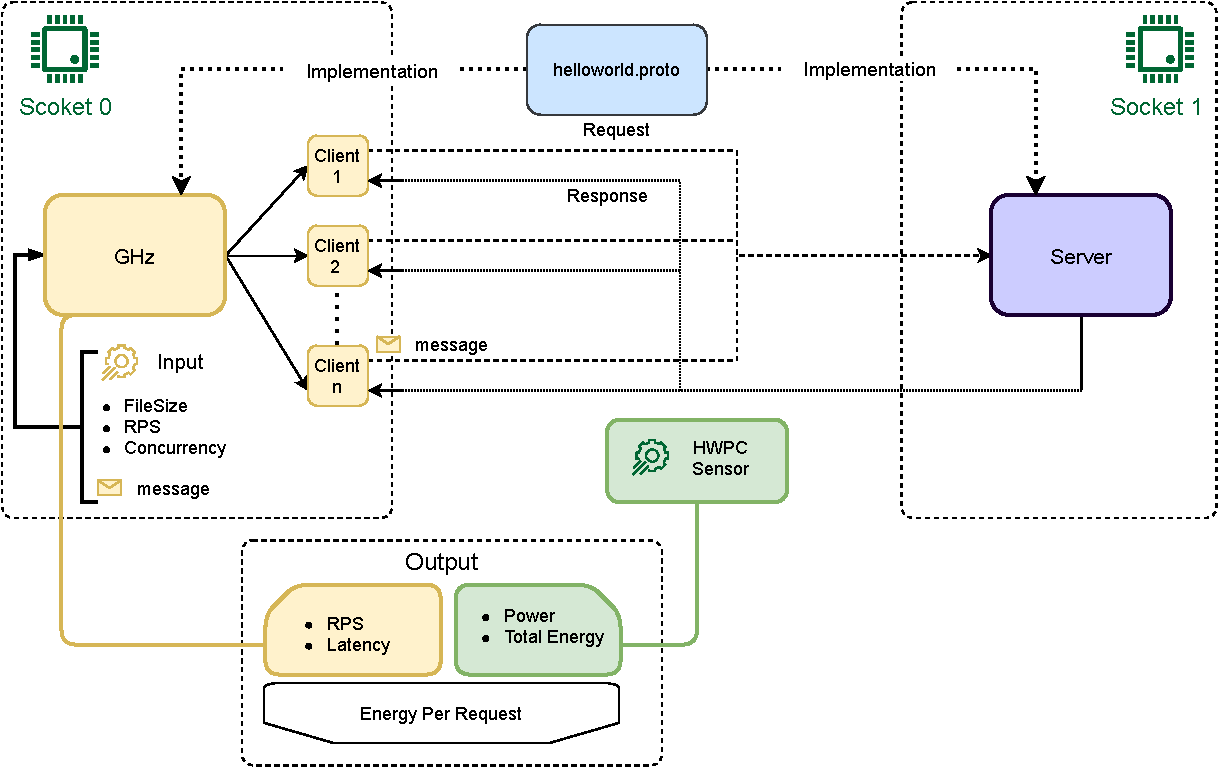
\includegraphics[width=.8\linewidth]{imgs/rpcprotocol}
    \end{center}
    \caption{Experimental software architecture.}\label{fig:rpcprotocol}
\end{figure}
Figure~\ref{fig:rpcprotocol} show the experimental protocol. We will use different messages inserted in the file \texttt{helloworld.proto}.
The rest of this part will be dedicated to explaining each aspect of the experiment.
\subsubsection{Measurement Context}
\paragraph{Hardware settings.}
All the experiments are run on the cluster \textsf{paravance} of the G5K platform.
This cluster comprises 72 identical machines equipped with 2 Intel Xeon E5-2630 V3, with 128\,GB of RAM.
For more accuracy, our SUT (\emph{System Under Test}) runs a minimal version of Debian\,9 (4.9.0 kernel version), which enforces the core processes required for our experiment.
Furthermore, we used Docker containers technology for the reproducibility of the experiments and the isolation of the servers.
\paragraph{Client \& server environments.}
To limit networks' impact on the experiments, we run both the client and the server on the same machine.
However, we isolate each part on a separate CPU socket to reduce the noise that the client might have on the server and \emph{vice-versa}.
To do so, for each iteration, we always run the same client on \textsf{socket\,0} and the server that we want to test on \textsf{socket\,1}.
Both the server and the client use the whole socket for their experiment.
In addition, all the additional services, such as the kernel and HwPC sensor, are run on \textsf{socket\,0}.
Therefore, the only process being executed in \textsf{socket\,1} is the server that we benchmark and monitor.

\subsubsection{Key Performance Metrics}
\paragraph{Energy measurements.}
To report on energy consumption, we used the \texttt{HWPC} sensor\footnote{\url{https://github.com/powerapi-ng/hwpc-sensor}}, based on Intel \texttt{RAPL} technology, one of the most accurate tools to measure the CPU's and DRAM's energy consumption~\cite{hackenberg2013power,hackenberg2015energy}.
For better accuracy, we ran the HwPC sensor with a frequency of 1~Hz, and we used the same machine for all the experiments to reduce the variability~\cite{ilsche_power_2015}.

\paragraph{Performances.}
For better accuracy and more details, We updated the open-source RPC benchmarking tool GHZ (\url{https://ghz.sh/}).
The modified version allows us to monitor the average power for each request from both the server and the client sides.
The new version is available in the repository.\footnote{\url{https://github.com/chakib-belgaid/energy_ghz}}

\subsubsection{Input Workload}
The purpose of the experiment is to analyze the behavior of different GRPC implementations.
Therefore, we have two kinds of workloads: \emph{number of clients} is the number of concurrent clients that we want to benchmark (handled by the GHZ client), and the \emph{payload} reflects the size of each request (varies from 50 Bytes up to 10 MB).
The client consumes the protocol description found in the file \texttt{helloworld.proto} to generate an implementation for the message and then forks multiple instances that send the same request to the server.

\subsubsection*{Candidates}
The server implementations are based on the official implementation by Google for most of the languages.
Each server uses 16 cores and is limited to 512\,MB of RAM.
Each implementation is packaged as a Docker image, allowing us to add new implementations easily.

\subsubsection{Extension}
For the sake of experimental extensibility, we provide a GitHub repository that contains the implementation of all our experiments.\footnote{\url{https://github.com/chakib-belgaid/energy_benchmarking_grpc2}}
Adding a new RPC \textbf{candidate} can be achieved by creating a new Docker image and putting it in a new folder named after the language.
As for the \textbf{workload}, it can be extended easily by adding new files in the folder \textbf{payload} and by changing the number of clients in the benchmarking tool.


\subsection{Results \& Findings}
\paragraph{Preparing the Data}
Before we start our Analysis, we will first clean the data from the outliers using the interquartile range (IQR) method~\cite{leys2013detecting}.
For each implementation, we will calculate the Q3 and Q1 of the population; then, we will exclude all the values outside the range
$ [Q1 - 1.5 \times IQR, Q3 + 1.5 \times IQR ]$.

\subsubsection{[\textsc{RQ}~1:] How do RPC implementations react to the number of clients?}

In this part, we will analyze the behavior of the different implementations regarding the number of clients.

\paragraph{Power behavior}
\begin{figure}[!htb]
    \begin{center}
        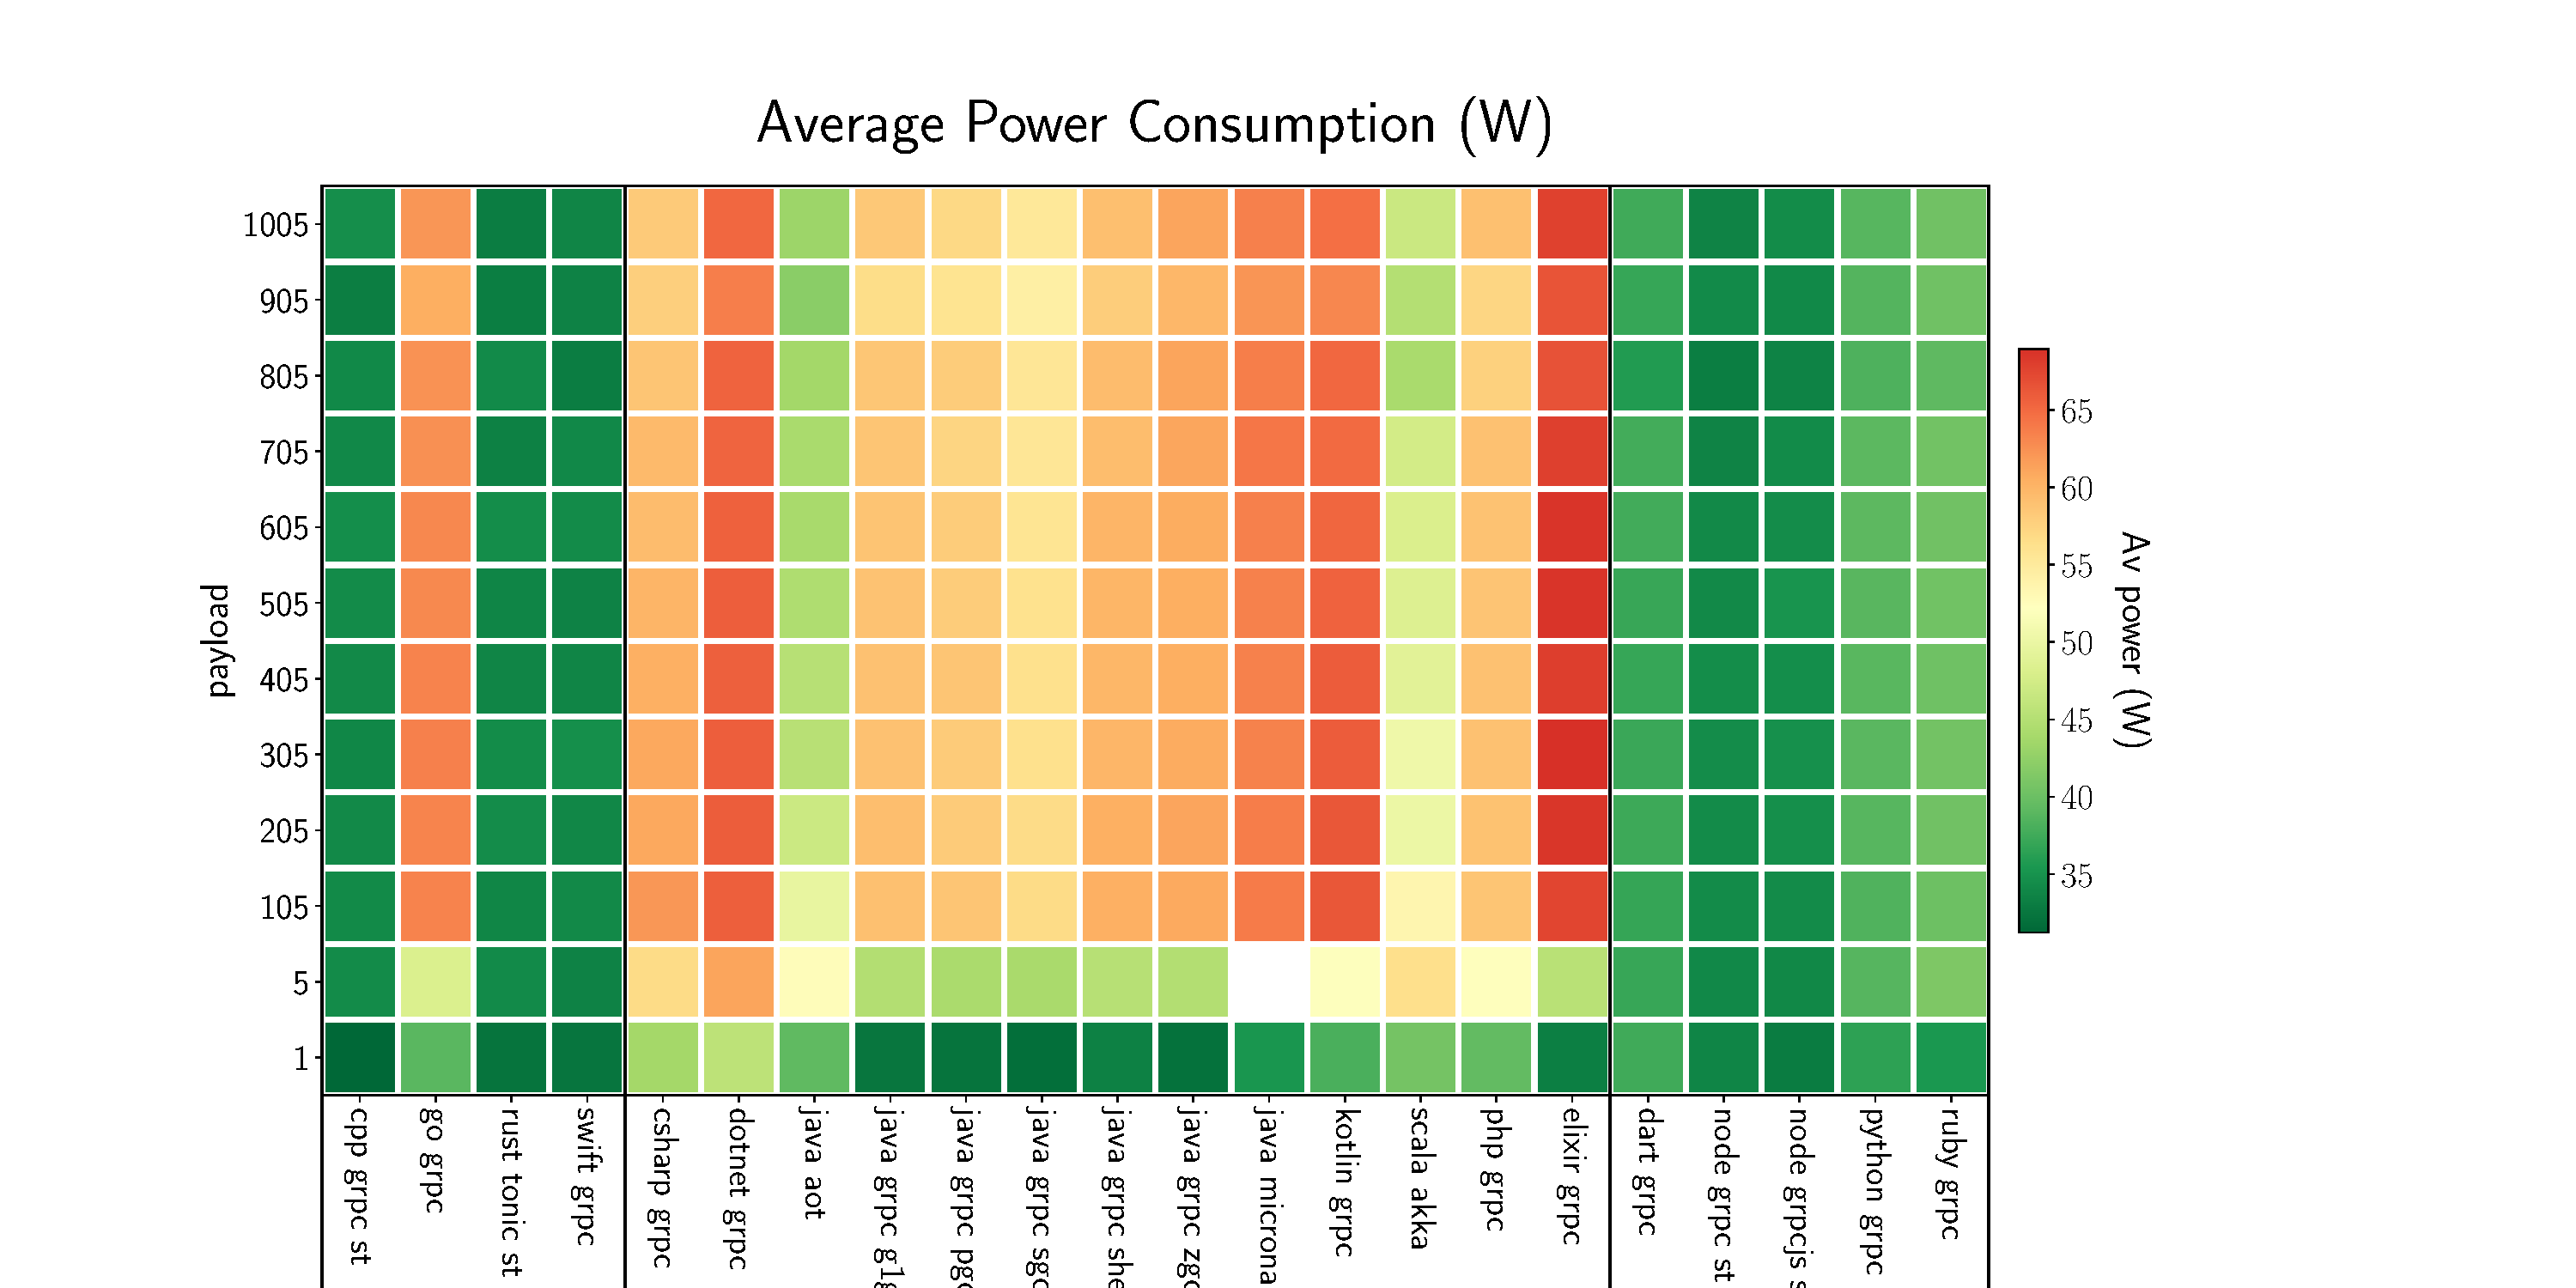
\includegraphics[width=1.2\linewidth]{imgs/power_consumption_clients}
    \end{center}
    \caption{Average power consumption based on the number of the clients}\label{fig:power_consumption_clients}
\end{figure}
First, we start with the overall power consumption for each server implementation.
Figure~\ref{fig:power_consumption_clients} shows a heatmap of the average power consumption of each implementation. As one can notice, there are two main scenarios. The first one is when the number of clients is lower than 100, which we will call \textsf{lite scenario}, and the second one, the \textsf{stressed scenario}, is when the number of clients is more exceeds 100.

\subparagraph{Lite scenario}
The benchmarked implementations can be grouped into two classes:
\begin{enumerate}
    \item \textsf{Energy-efficient frameworks} where most of the framework's power consumption is around 33 Watts.
    \item \textsf{Energy-greedy frameworks} where the average power consumption is higher than 45 Watts.
\end{enumerate}
In each programming category, we observe both energy-efficient and energy-greedy behaviors.
Therefore, we conclude that it depends more on the library's implementation than the programming language category.
Scala and Kotlin are excellent examples to support this hypothesis, as both run on the same virtual machine as Java (OpenJDK 16.1).
However, their average power is 130\% higher than the Java implementation.

\subparagraph{Stressed scenario}
Although the same classes remained the same, not all languages had the same evolution. Here we can observe a correlation with the category of the programming language rather than the implementation itself.
We can quickly point out that the average amount of power used by VM-based languages doubles when they have more than 100 clients simultaneously.
Except for PHP, all the interpreted and compiled languages preserved their energetic behavior.
Our hypothesis points to the JIT since it compiles the code and makes it run faster, hence stressing the CPU.
An interesting behavior has been noticed for the GraalVM: decreasing energy consumption when increasing the number of clients.
This is related to the performance drop, probably due to the bottleneck situation where the GraalVM could not handle more than 100 clients simultaneously.

\paragraph{Performance Behaviour}
this paragraph will cover the number of requests per second processed per server without looking at its energy.
Here, we consider three observable variables:
\begin{itemize}
    \item \textsf{Satisfaction ratio}: how many requests have been satisfied among the total requests,
    \item \textsf{Request Per Seconds}: The number of requests that have been answered from the server,
    \item \textsf{Tail Latency at 99\%}: one of the best metrics to evaluate the performances of a server.
\end{itemize}

\subparagraph{Satisfaction ratio}
Most of the considered frameworks satisfy all the requests by reducing the number of requests per second or increasing the processing time.
However, some frameworks, such as Dart or Scala, have taken a different approach, maintaining a specific latency limit even if not all requests are answered.
Furthermore, we tend to observe this behavior among other frameworks, such as Python or Asynchronous NodeJS, when the number of clients exceeds 800. To dive more into this behavior, the reader can refer to the following  GitHub repository \url{https://github.com/chakib-belgaid/grpc_analysis}

\subparagraph{RPS}

\begin{figure}[!hbt]
    \begin{center}
        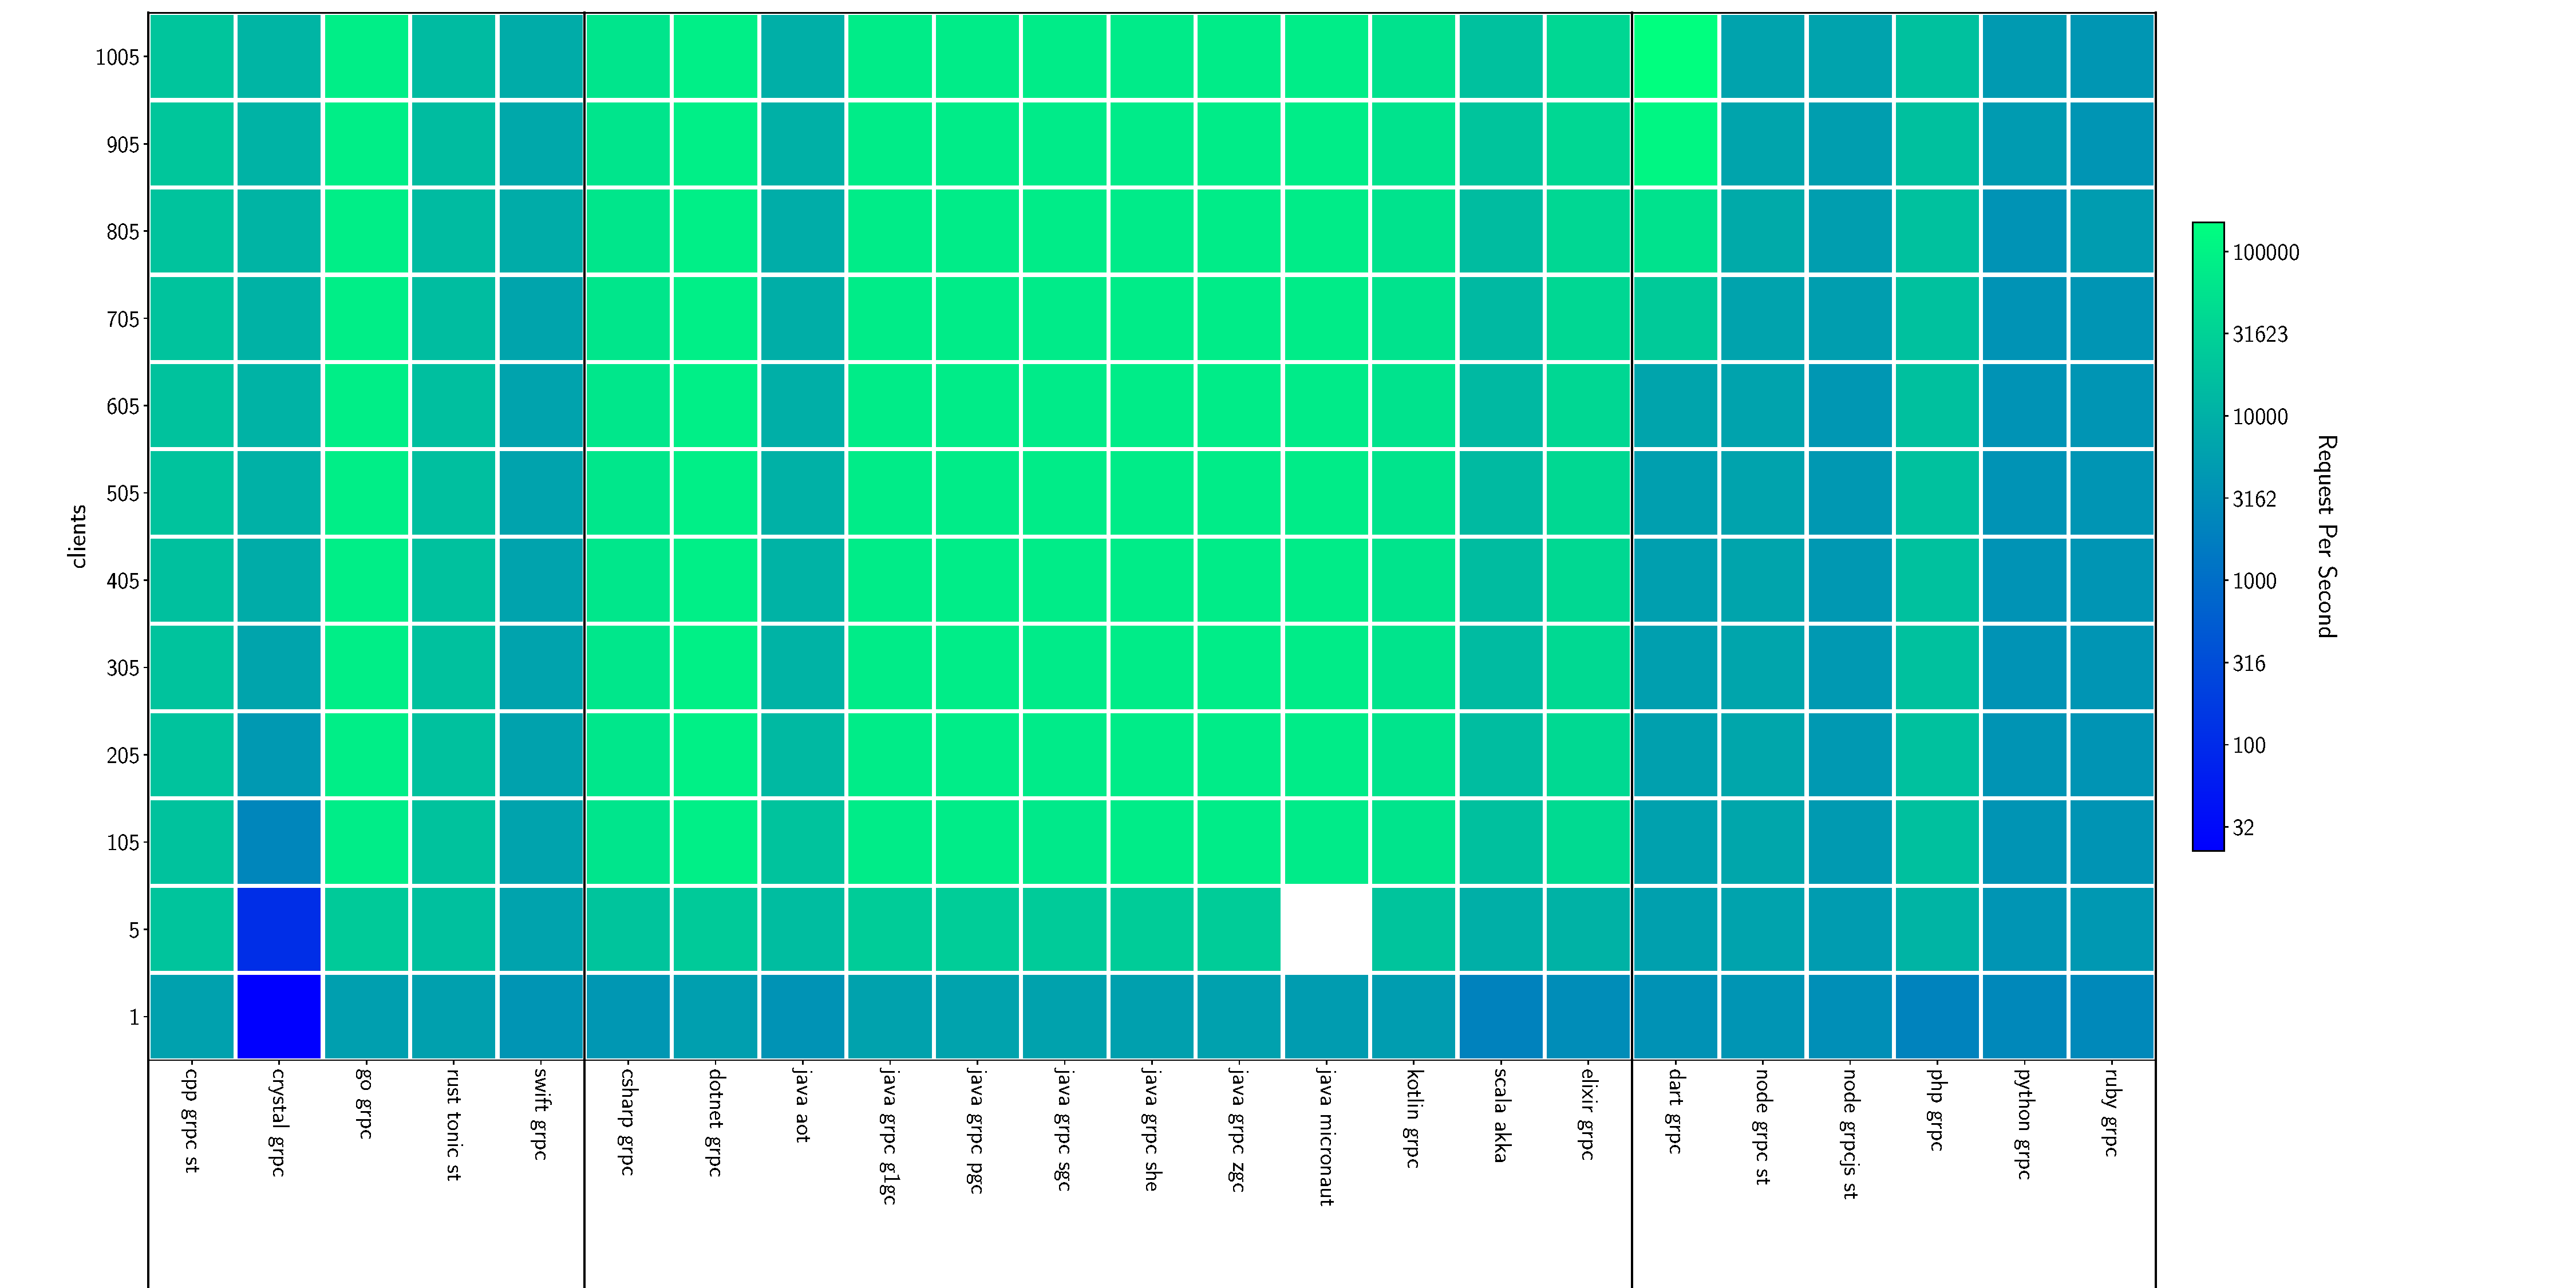
\includegraphics[width=1.2\linewidth]{imgs/rps_clients}
    \end{center}
    \caption{Number of requests per second based on the number of clients}\label{fig:rps_clients}
\end{figure}
%  TODO : REname the frameworks based on their dockerfile 

Figure~\ref{fig:rps_clients} presents the number of requests per second for each implementation. The heatmap is colored with a logarithmic scale to visualize the results better.
As one can observe, most of the servers hit their RPS limit after five clients and 100 clients for VM-based servers, and after this, the number keeps constant, decreasing the average RPS per client.
.Net server is the most performant, followed by Java and Go, while Python and Ruby are the least performant.

\subparagraph{Tail Latency}
Even if the number of requests per second increases, that does not mean the latency will go down.
As one can notice in figure~\ref{fig:tail99_clients}, until the 1000 clients, Go provides the least latency besides.Net.
GraalVM provides the highest average latency.
However, Dart tends to become slower when we increase the number of clients until we pass the 600 simultaneous clients, and then it changes its behavior. Instead of satisfying most of the requests, it notifies the clients directly that the server is saturated, resulting in a drop in satisfaction ratio and an amelioration in average latency.

\begin{figure}[!hbt]
    \begin{center}
        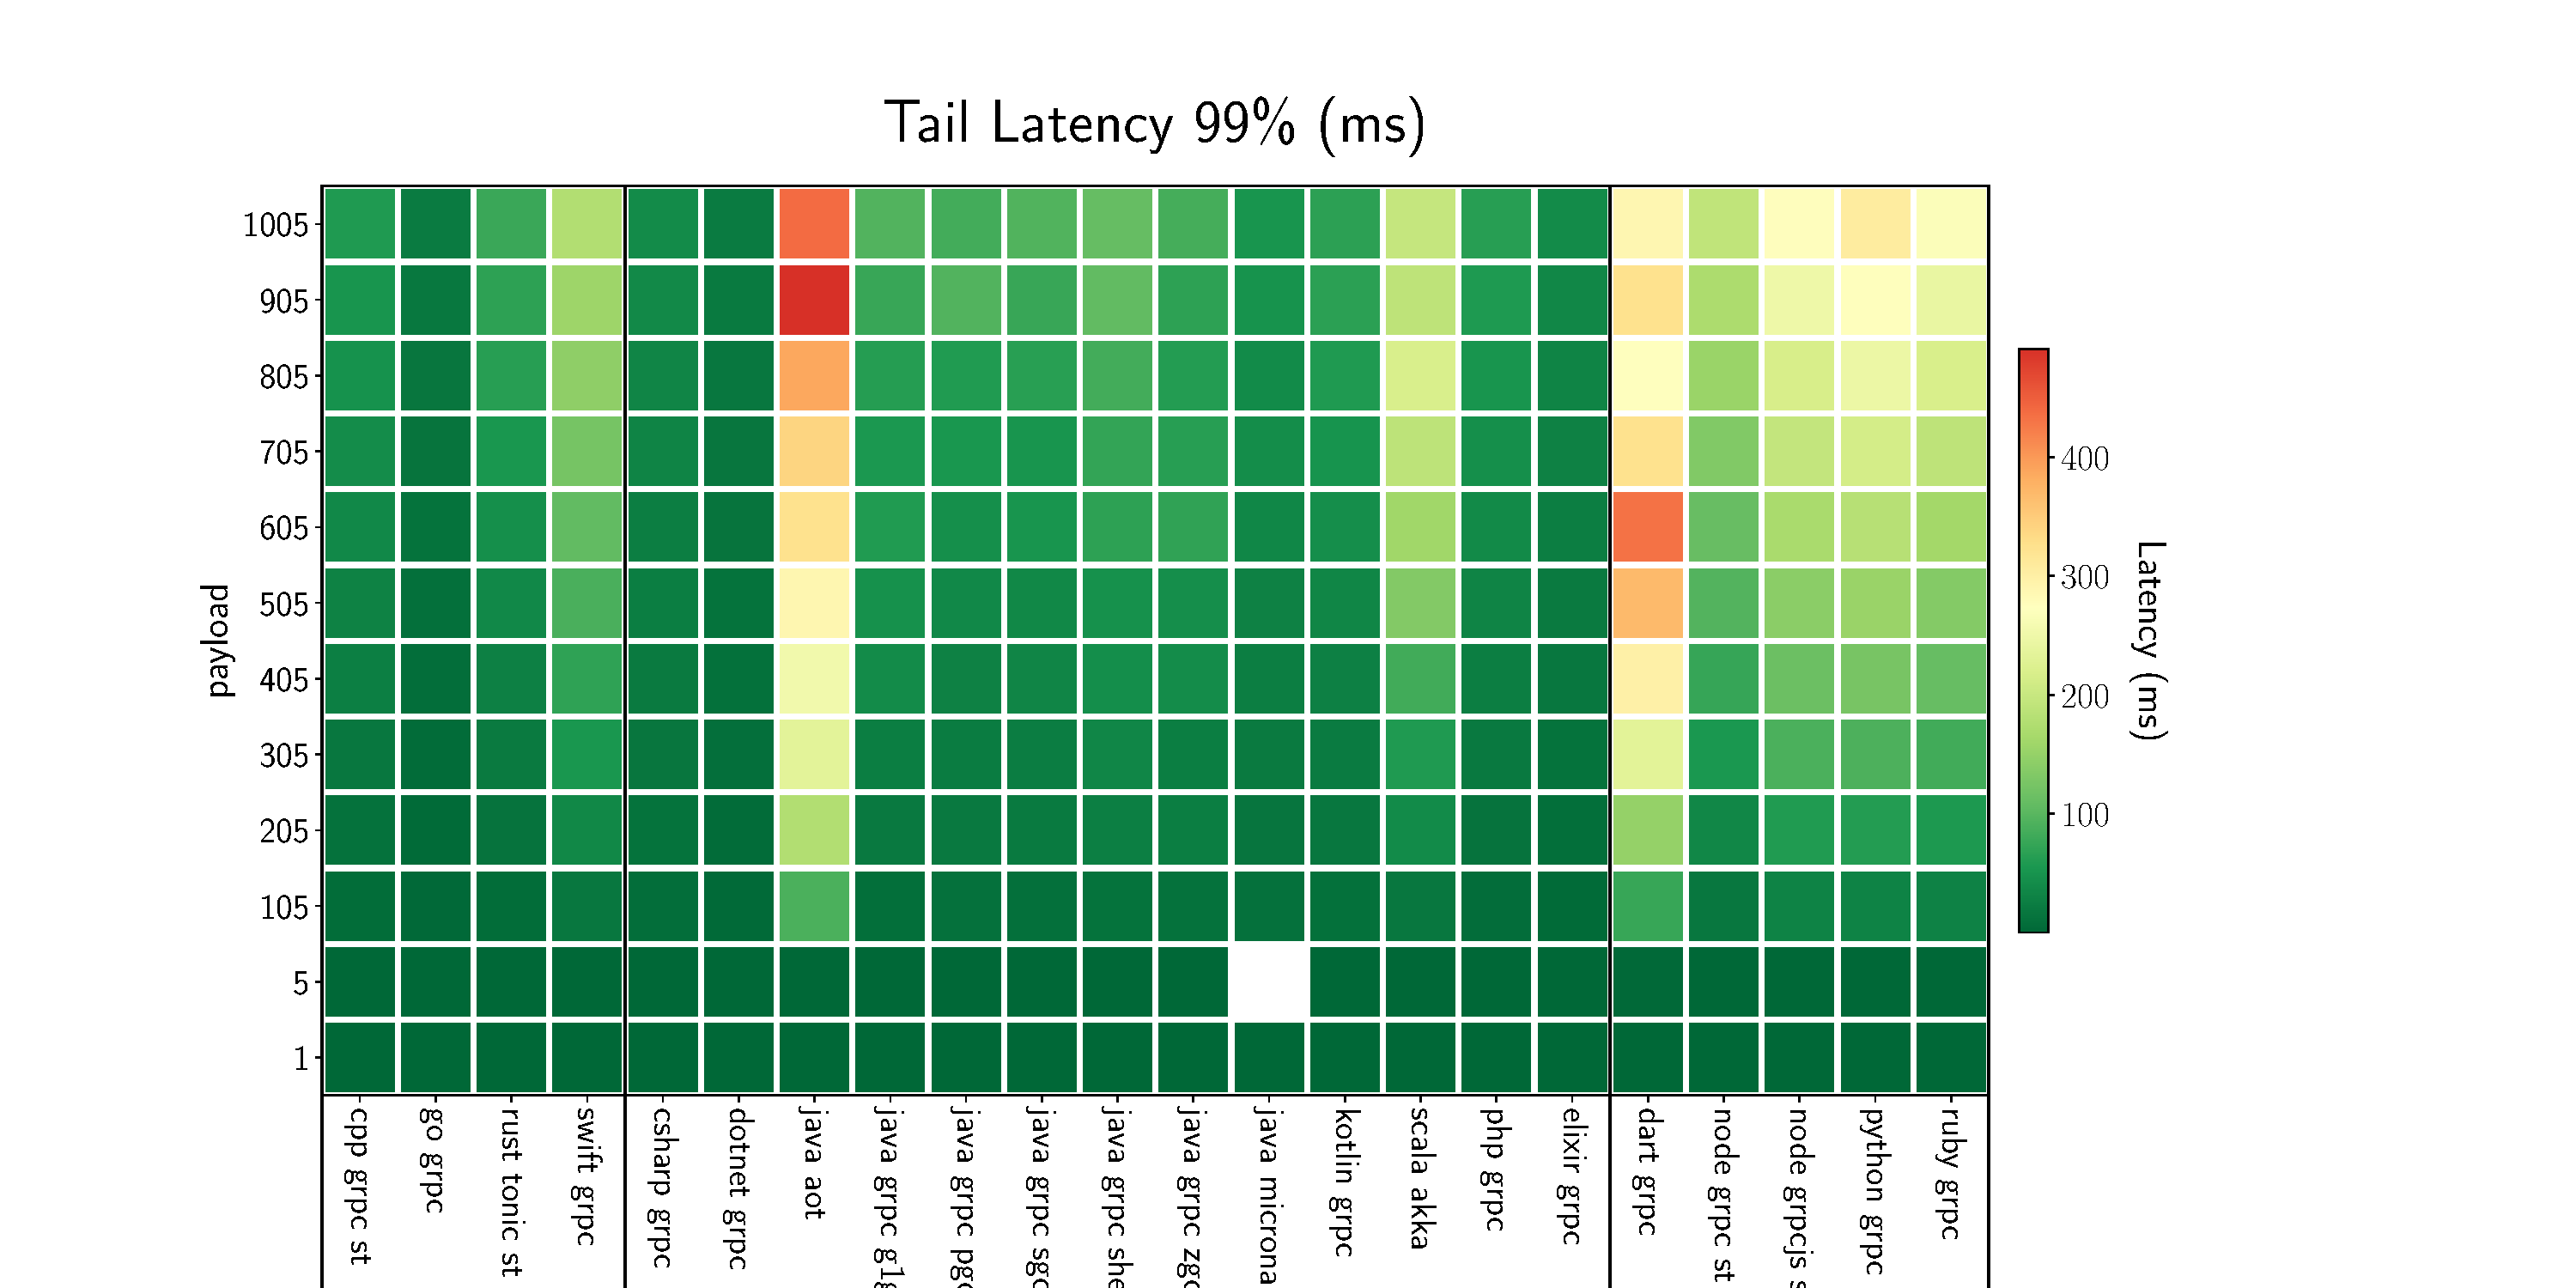
\includegraphics[width=1.2\linewidth]{imgs/tail99_clients}
    \end{center}
    \caption{Tail latency (99\%) based on the number of clients}\label{fig:tail99_clients}
\end{figure}



\paragraph{Energy Per Request}
\begin{figure}[!hbt]
    \begin{center}
        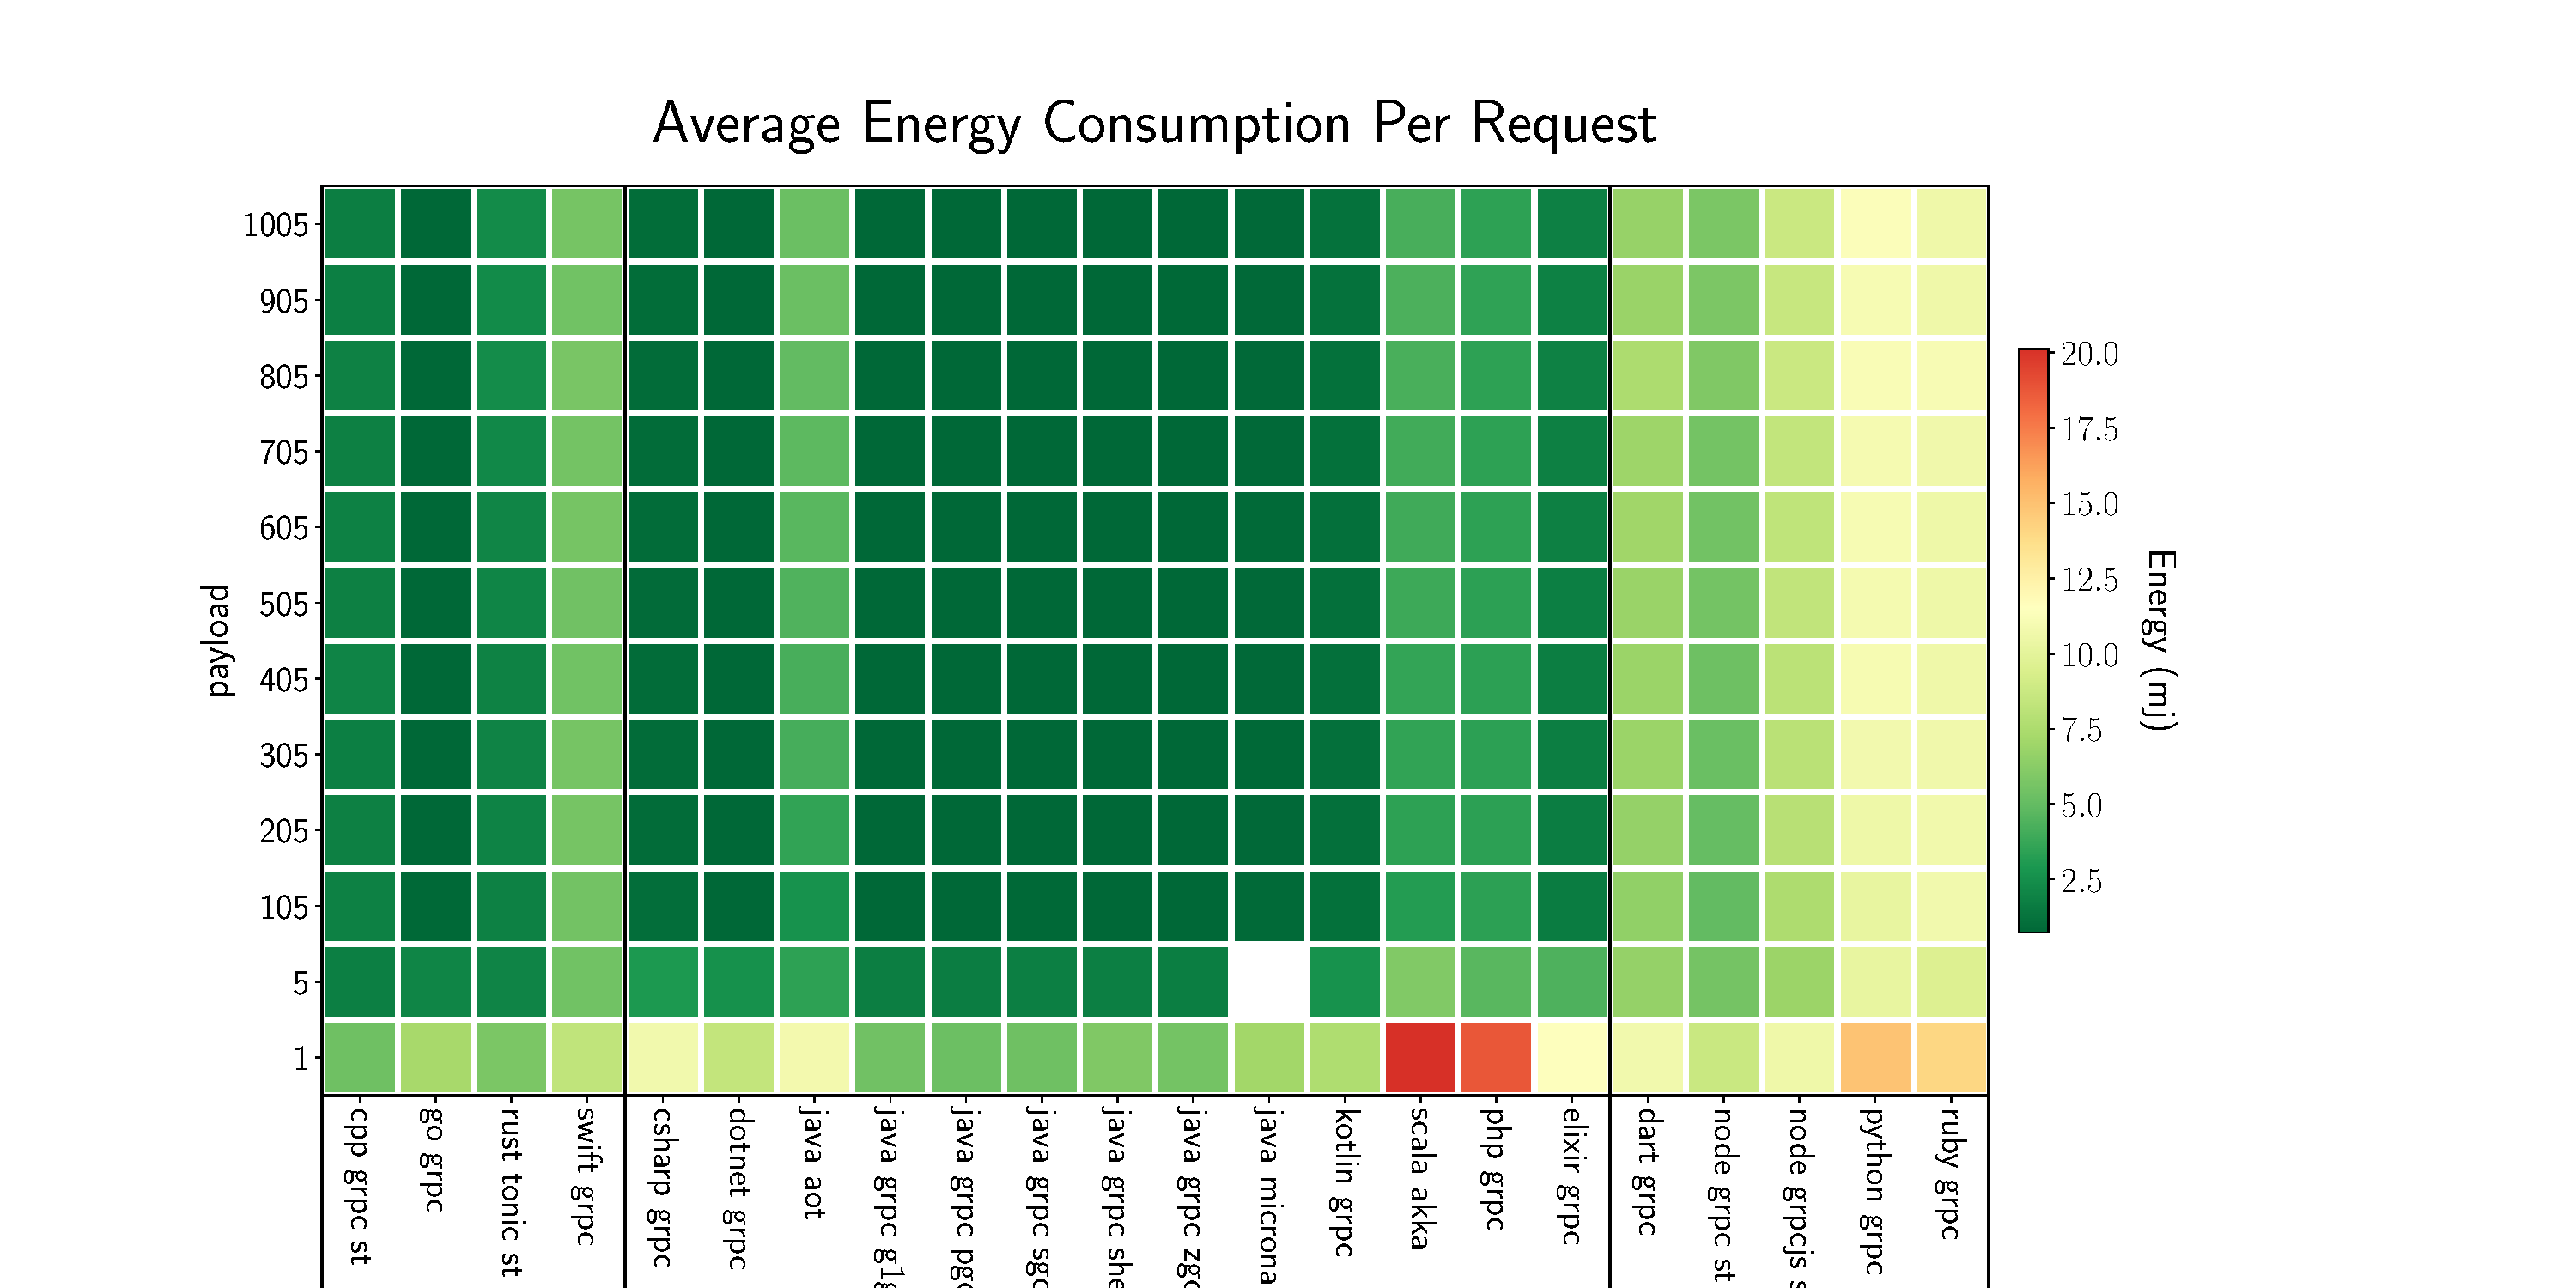
\includegraphics[width=1.2\linewidth]{imgs/energy_cost_clients}
    \end{center}
    \caption{The cost of a single request based on the number of clients (mJ)}\label{fig:energy_cost_clients}
\end{figure}
After separating the energy and the performances, we have seen that most performance servers tend to be energy-greedy, so we propose investigating this trade-off between energy and performance.
To do so, we report the average cost of a single request in millijoules in Figure~\ref{fig:energy_cost_clients}.

Except for GraalVM (aka Java AOT), the cost of the single request decreases when we add more clients.Java, .Net, and go are the most energy efficient, while Python and Ruby may cost up to 10x more.
Despite its low power, textsfCrystal exhibits greedy behavior when dealing with requests from fewer clients. Such behavior is caused by the low number of requests per second, which also results in high latency.
Therefore, we conclude that the number of clients does not significantly impact energy consumption.
Then, we study how the payload size of the requests impacts the energy consumption of the framework.


% \paragraph{Synthesis}:
% Depending on the number of clients, most frameworks exhibit two distinct behaviors. When dealing with a small number of clients, frameworks, regardless of programming category, tend to be energy-efficient and performant.
% However, as the number of clients grows, the frameworks become more energy-hungry and less performant. Interpreted languages suffer the most, particularly in terms of latency and the cost of a single request.
% \textsf{Crystal}, interestingly, acted. It behaves oppositely. The cost of a single request increases as the number of clients decreases.


\subsubsection{\textsc{RQ}~2: How do RPC implementations consume energy concerning the size of the incoming request?}

The purpose of this question is to study the energy consumption of the RPC server when transferring large objects.
To do so, we send $80,000$ requests to the server whose size scales from 10 bytes up to 10 Megabytes, resulting in $10,000$ requests per size per server.
To eliminate extra factors, we let the server handle the rate at which it can answer each request.
However, we put a 20 seconds timeout deadline for each category of requests.
Therefore, our boundary condition is only the number of requests received by the server.
For this experiment, we investigate four observable variables:
\begin{enumerate}
    \item the \textsf{average power consumption} during the scenario indicates the overall behavior of the server when working for long durations, Figure~\ref{fig:power_consumption_payload},
    \item the \textsf{tail latency} for the 99th percentile, which indicates how efficient the server is, Figure~\ref{fig:tail99_payload}
    \item the \textsf{average number of requests per second}, which indicates the average number of clients that the server can handle, Figure~\ref{fig:rps_payload}
    \item the \textsf{average energy cost} of a single request: unlike the first indicator, this one shows how green the implementation is, considering performance, Figure~\ref{fig:energy_cost_payload}
\end{enumerate}

% NOTE : discuss this with Romain later (90% chances that it is not needed)
% \paragraph{overall analysis}
% 




% \begin{table}\caption{Correlation or something}
%     \centering
%     \pgfplotstabletypeset[color cells]{
%         % Language    , Power~RPS  ,Power~energy~request, RPS~Tail~latency , RPS~Energy~request     
%         cpp~st,-0.68,0.89,-1.00,-0.86
%         crystal,0.40,-0.40,-0.80,-1.00
%         go,-0.75,1.00,-0.89,-0.75
%         rust~tonic~st,-0.05,0.62,-0.98,-0.57
%         swift,-0.17,0.31,-1.00,-0.88
%         csharp,-0.14,0.04,-0.96,-0.96
%         dotnet,-1.00,0.96,-0.89,-0.96
%         javaaot,-0.57,0.79,-0.96,-0.93
%         java~g1gc,-0.61,0.71,-0.89,-0.71
%         java~pgc,-0.79,0.68,-0.86,-0.89
%         java~sgc,-0.79,0.79,-1.00,-0.82
%         java~she,-0.82,0.50,-0.86,-0.79
%         java~zgc,-0.75,0.89,-0.68,-0.89
%         java~micronaut,-0.14,0.00,-0.86,-0.89
%         kotlin,-0.68,0.89,-0.93,-0.86
%         scala,0.77,-0.60,-0.83,-0.94
%         elixir,-0.93,0.93,-0.98,-1.00
%         dart,-0.76,0.76,-0.95,-0.95
%         node~st,-0.86,0.86,-1.00,-1.00
%         node~js~st,-0.89,0.96,-0.93,-0.96
%         php,-0.96,0.96,-0.89,-1.00
%         python,-0.29,0.86,-0.96,-0.68
%         ruby,-0.43,0.68,-1.00,-0.89
%     }

% \end{table}

\newcommand\high[1]{\textcolor{red}{ #1}}
\newcommand\average[1]{\textcolor{orange}{ #1}}
\newcommand\low[1]{\textcolor{olive}{ #1}}
\newcommand\nocorr[1]{\textcolor{teal}{ #1}}
\begin{table*}[!htb]

    \raggedright
    \resizebox{\linewidth}{!}{
        \begin{tabular}{|l|c|c|c|c|c|}
            \toprule
            Language       & Power / RPS   &  Power / Tail latency & Power / energy per request & RPS / Tail latency & RPS/ Energy per request \\
            \midrule
            cpp grpc st    & \average{-0.68} & \average{0.68 }& \high{0.89}               & \high{-1.00}       & \high{-0.86}            \\
            crystal grpc   & \average{0.40}  & \average{-0.20}& \average{-0.40}            & \high{-0.80}       & \high{-1.00}            \\
            go grpc        & \high{-0.75}    & \average{0.64 }& \high{1.00}               & \high{-0.89}       & \high{-0.75}            \\
            rust tonic st  & \nocorr{-0.05}  &  \nocorr{0.02 }& \average{0.62}            & \high{-0.98}       & \average{-0.57}         \\
            swift grpc     & \nocorr{-0.17}  &  \nocorr{0.17 }& \low{0.31}                & \high{-1.00}       & \high{-0.88}            \\
            csharp grpc    & \nocorr{-0.14} &  \nocorr{0.21 }& \nocorr{0.04}             & \high{-0.96}       & \high{-0.96}            \\
            dotnet grpc    & \nocorr{-1.00}  &  \high{0.89 }& \high{0.96}               & \high{-0.89}       & \high{-0.96}            \\
            java aot       & \average{-0.57} & \average {0.68 }& \high{0.79}               & \high{-0.96}       & \high{-0.93}            \\
            java grpc g1gc & \average{-0.61} &  \average{0.54 }& \average{0.71}            & \high{-0.89}       & \high{-0.71}            \\
            java grpc pgc  & \high{-0.79}    &  \low{0.46 }& \average{0.68}            & \high{-0.86}       & \high{-0.89}            \\
            java grpc sgc  & \high{-0.79}    &  \high{0.79 }& \high{0.79}               & \high{-1.00}       & \high{-0.82}            \\
            java grpc she  & \high{-0.82}    &  \high{0.96 }& \average{0.50}            & \high{-0.86}       & \high{-0.79}            \\
            java grpc zgc  & \high{-0.75}    &  \high{0.79 }& \high{0.89}               & \high{-0.68}       & \high{-0.89}            \\
            java micronaut & \nocorr{-0.14}  &  \nocorr{-0.18}& \nocorr{0.00}             & \high{-0.86}       & \high{-0.89}            \\
            kotlin grpc    & \average{-0.68} &  \average{0.68 }& \high{0.89}               & \high{-0.93}       & \high{-0.86}            \\
            scala akka     & \high{0.77}    &  \low{-0.49}& \average{-0.60}            & \high{-0.83}       & \high{-0.94}            \\
            elixir grpc    & \high{-0.93}    &  \high{0.90 }& \high{0.93}               & \high{-0.98}       & \high{-1.00}            \\
            dart grpc      & \high{-0.76}    &  \high{0.76 }& \high{0.76}               & \high{-0.95}       & \high{-0.95}            \\
            node grpc st   & \high{-0.86}    &  \high{0.86 }& \high{0.86}               & \high{-1.00}       & \high{-1.00}            \\
            node grpcjs st & \high{-0.89}    &  \high{0.75 }& \high{0.96}               & \high{-0.93}       & \high{-0.96}            \\
            php grpc       & \high{-0.96}    &  \high{0.82 }& \high{0.96}               & \high{-0.89}       & \high{-1.00}            \\
            python grpc    & \low{-0.29}     &  \low{0.32 }& \high{0.86}               & \high{-0.96}       & \high{-0.68}            \\
            ruby grpc      & \low{-0.43}     &  \low{0.40 }& \average{0.68}            & \high{-1.00}       & \high{-0.89}            \\
            \bottomrule
        \end{tabular}
    }
    \caption{Corellation between multiple metrics for each server }
    \label{table:correlation}
\end{table*}
% in order to reduce the space of research, we processed to do a correlation test between the different variables. We used the Pearson Spearman rank correlation~\cite{zar2005spearman}. 

% Table~\ref{table:correlation} presents the correlation between the different observable variables. As one can see,  There is a high correlation between the number of requests, the 99\% tail latency, and the average energy cost. This means that the more requests are answered, the less energy is consumed, and the more latency is observed. However, the correlation between the average power consumption and the other variables is low, which means that the power consumption is not directly related to the other variables.  
% As one can see, except for rust-based implementation, the correlation between the energy consumption per request and the tail latency was extremely high. 
% Therefore, we will focus on two main variables 
% \begin{itemize}
%     \item average power consumption - that will represent the energetic behavior of the server 
%     \item average request per second: that will be our representative variable to estimate the performance 
% \end{itemize}

% We chose these two variables because they are both expressed in seconds, which will narrow our analysis to the present behavior of the server at any given time and not along the whole execution process.  

% As one can notice in the first column of table~\ref{table:correlation}
% There are three main categories of servers. 
% \begin{enumerate}
%     \item Positive correlation between the energy and performance :  
% \end{enumerate}




% \paragraph{metric based analysis}

\begin{figure}[!hbt]
    \begin{center}
        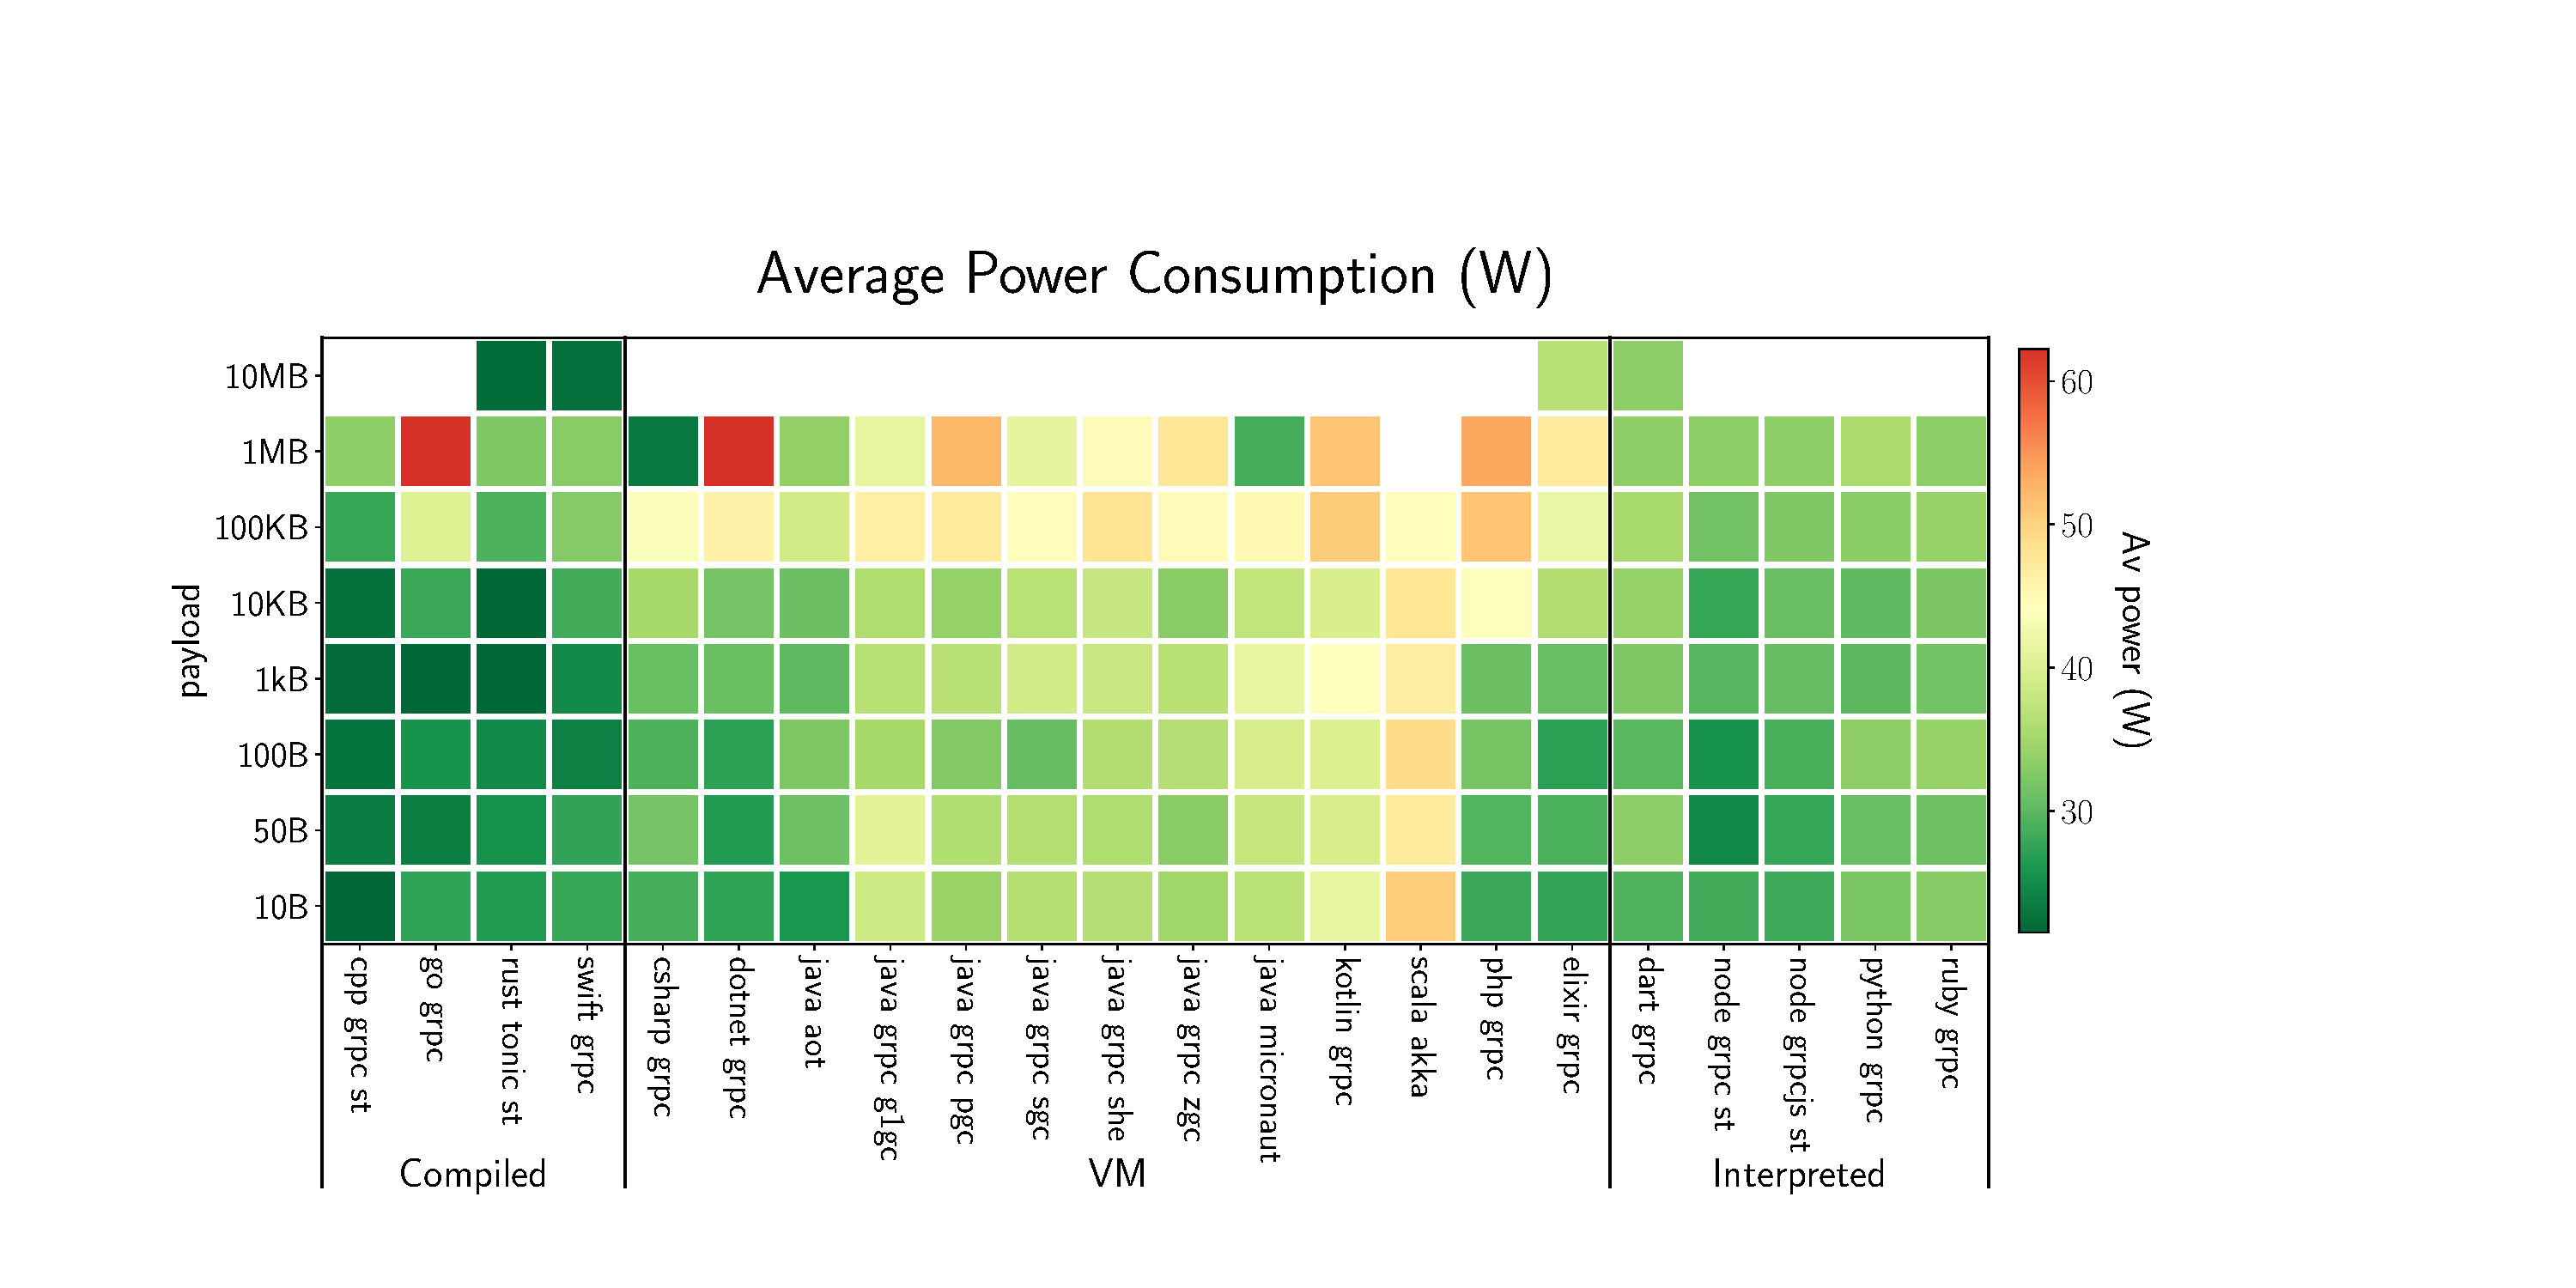
\includegraphics[width=1.2\linewidth]{imgs/power_consumption_payload}
    \end{center}
    \caption{Average power consumption based on the request size}\label{fig:power_consumption_payload}
\end{figure}


\begin{figure}[!hbt]
    \begin{center}
        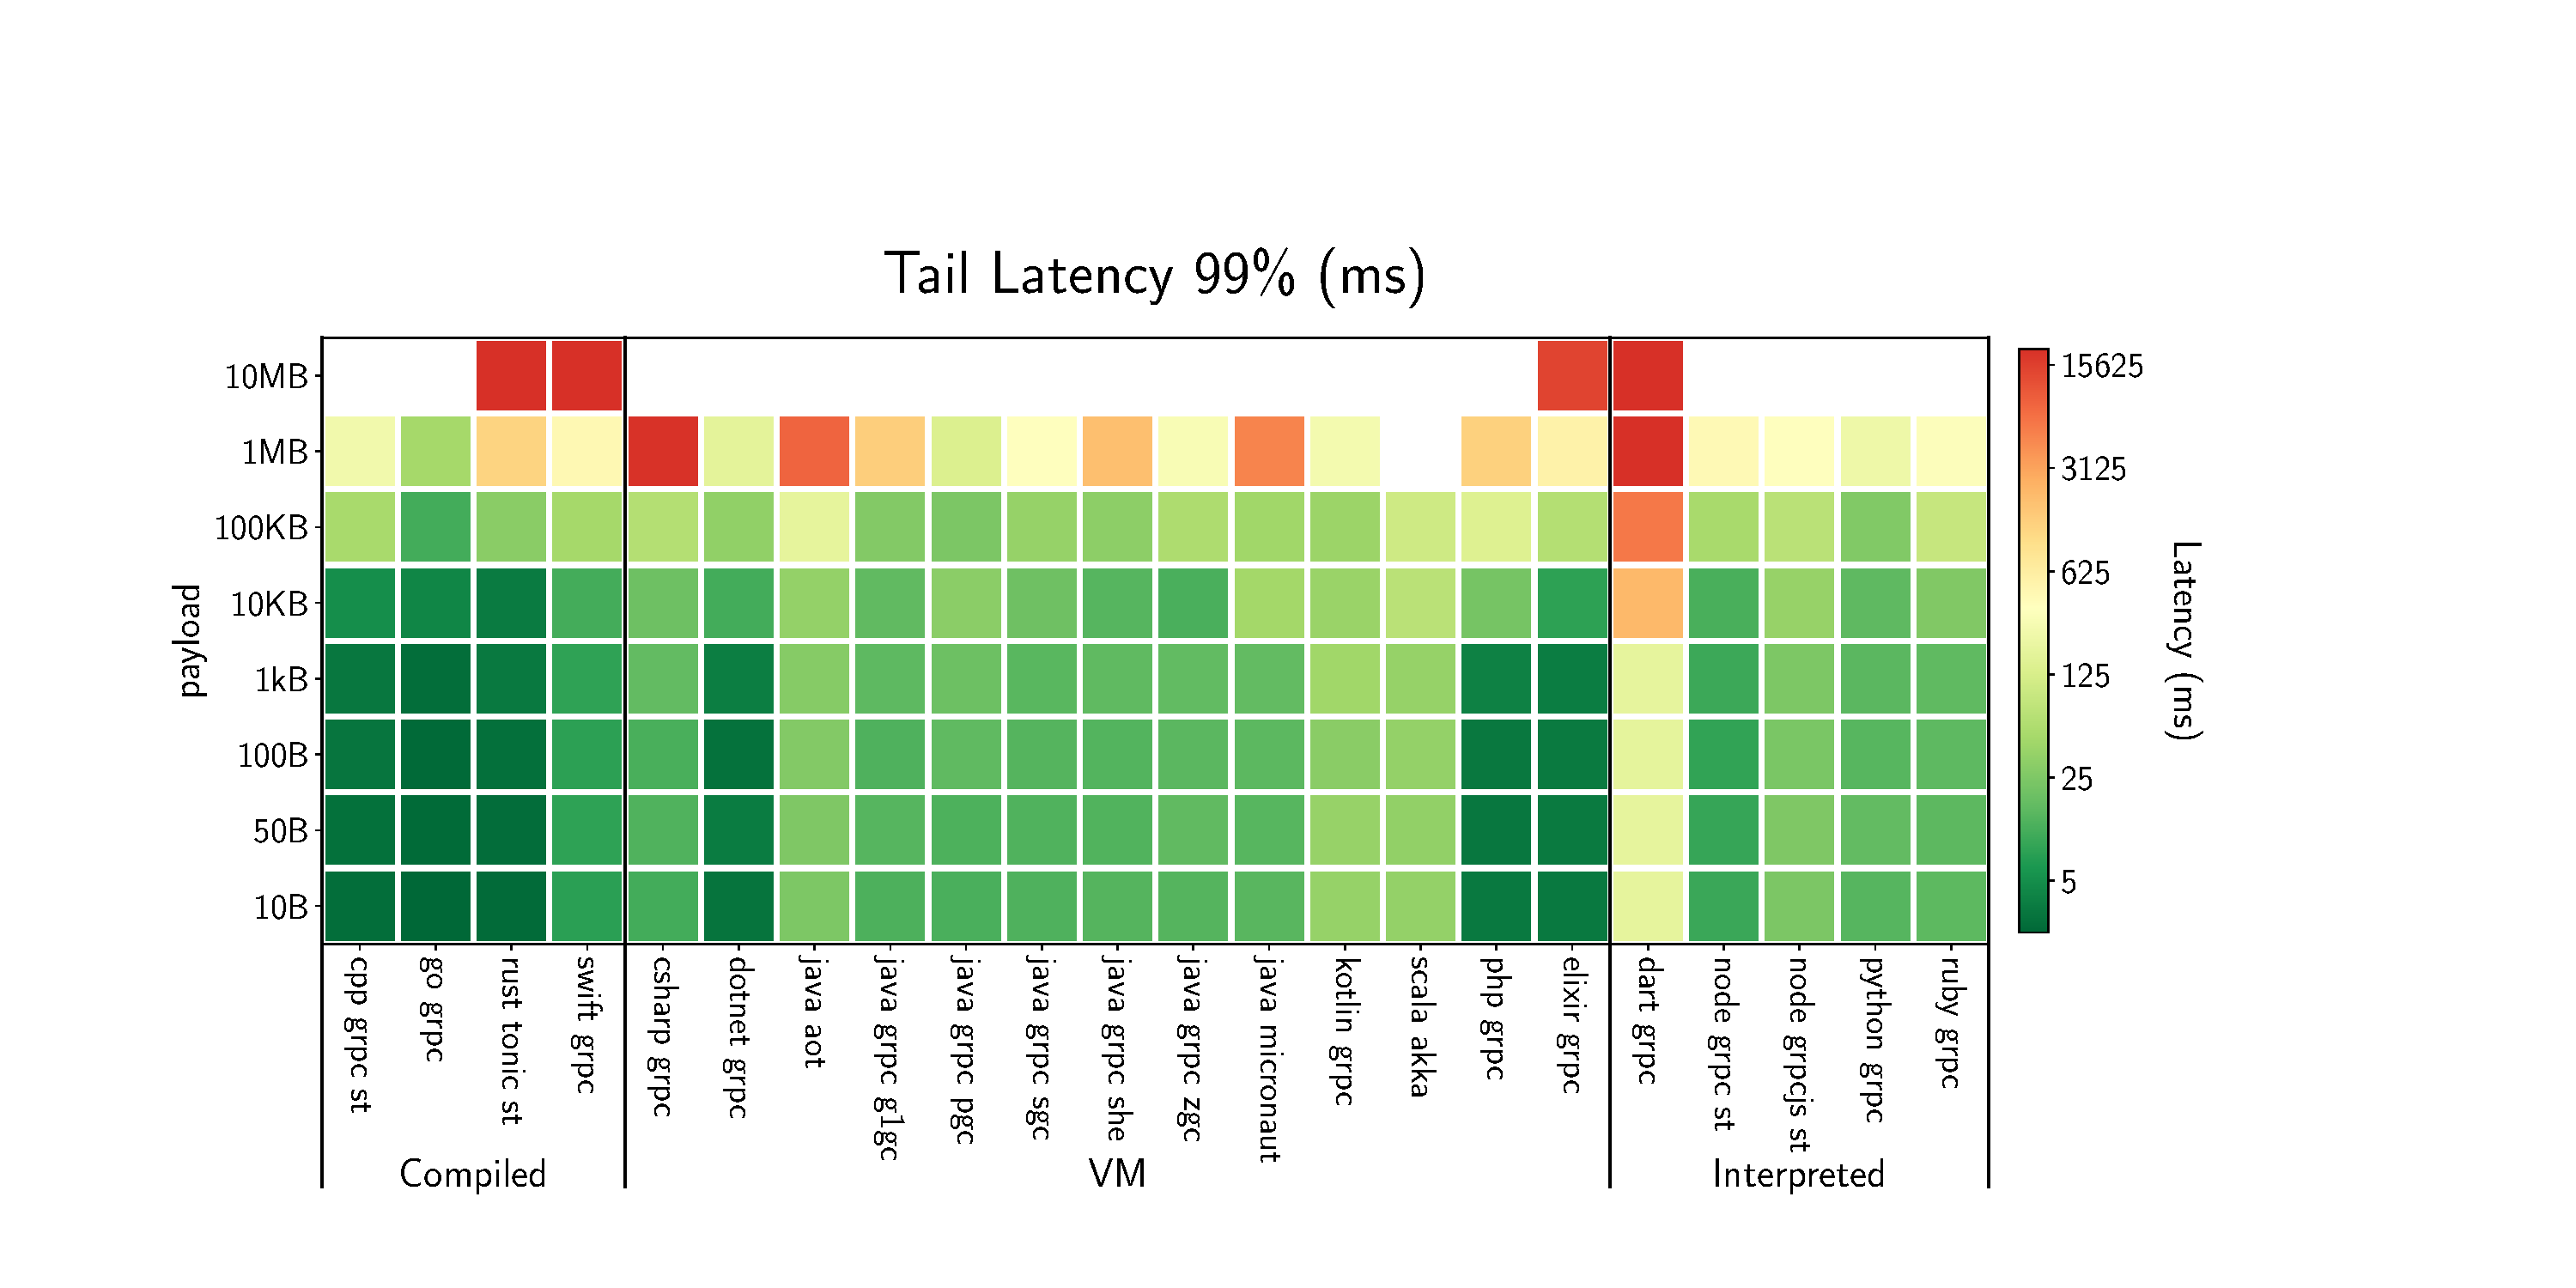
\includegraphics[width=1.2\linewidth]{imgs/tail99_payload}
    \end{center}
    \caption{Tail latency (99\%) based on the request size}\label{fig:tail99_payload}
\end{figure}

\begin{figure}[!hbt]
    \begin{center}
        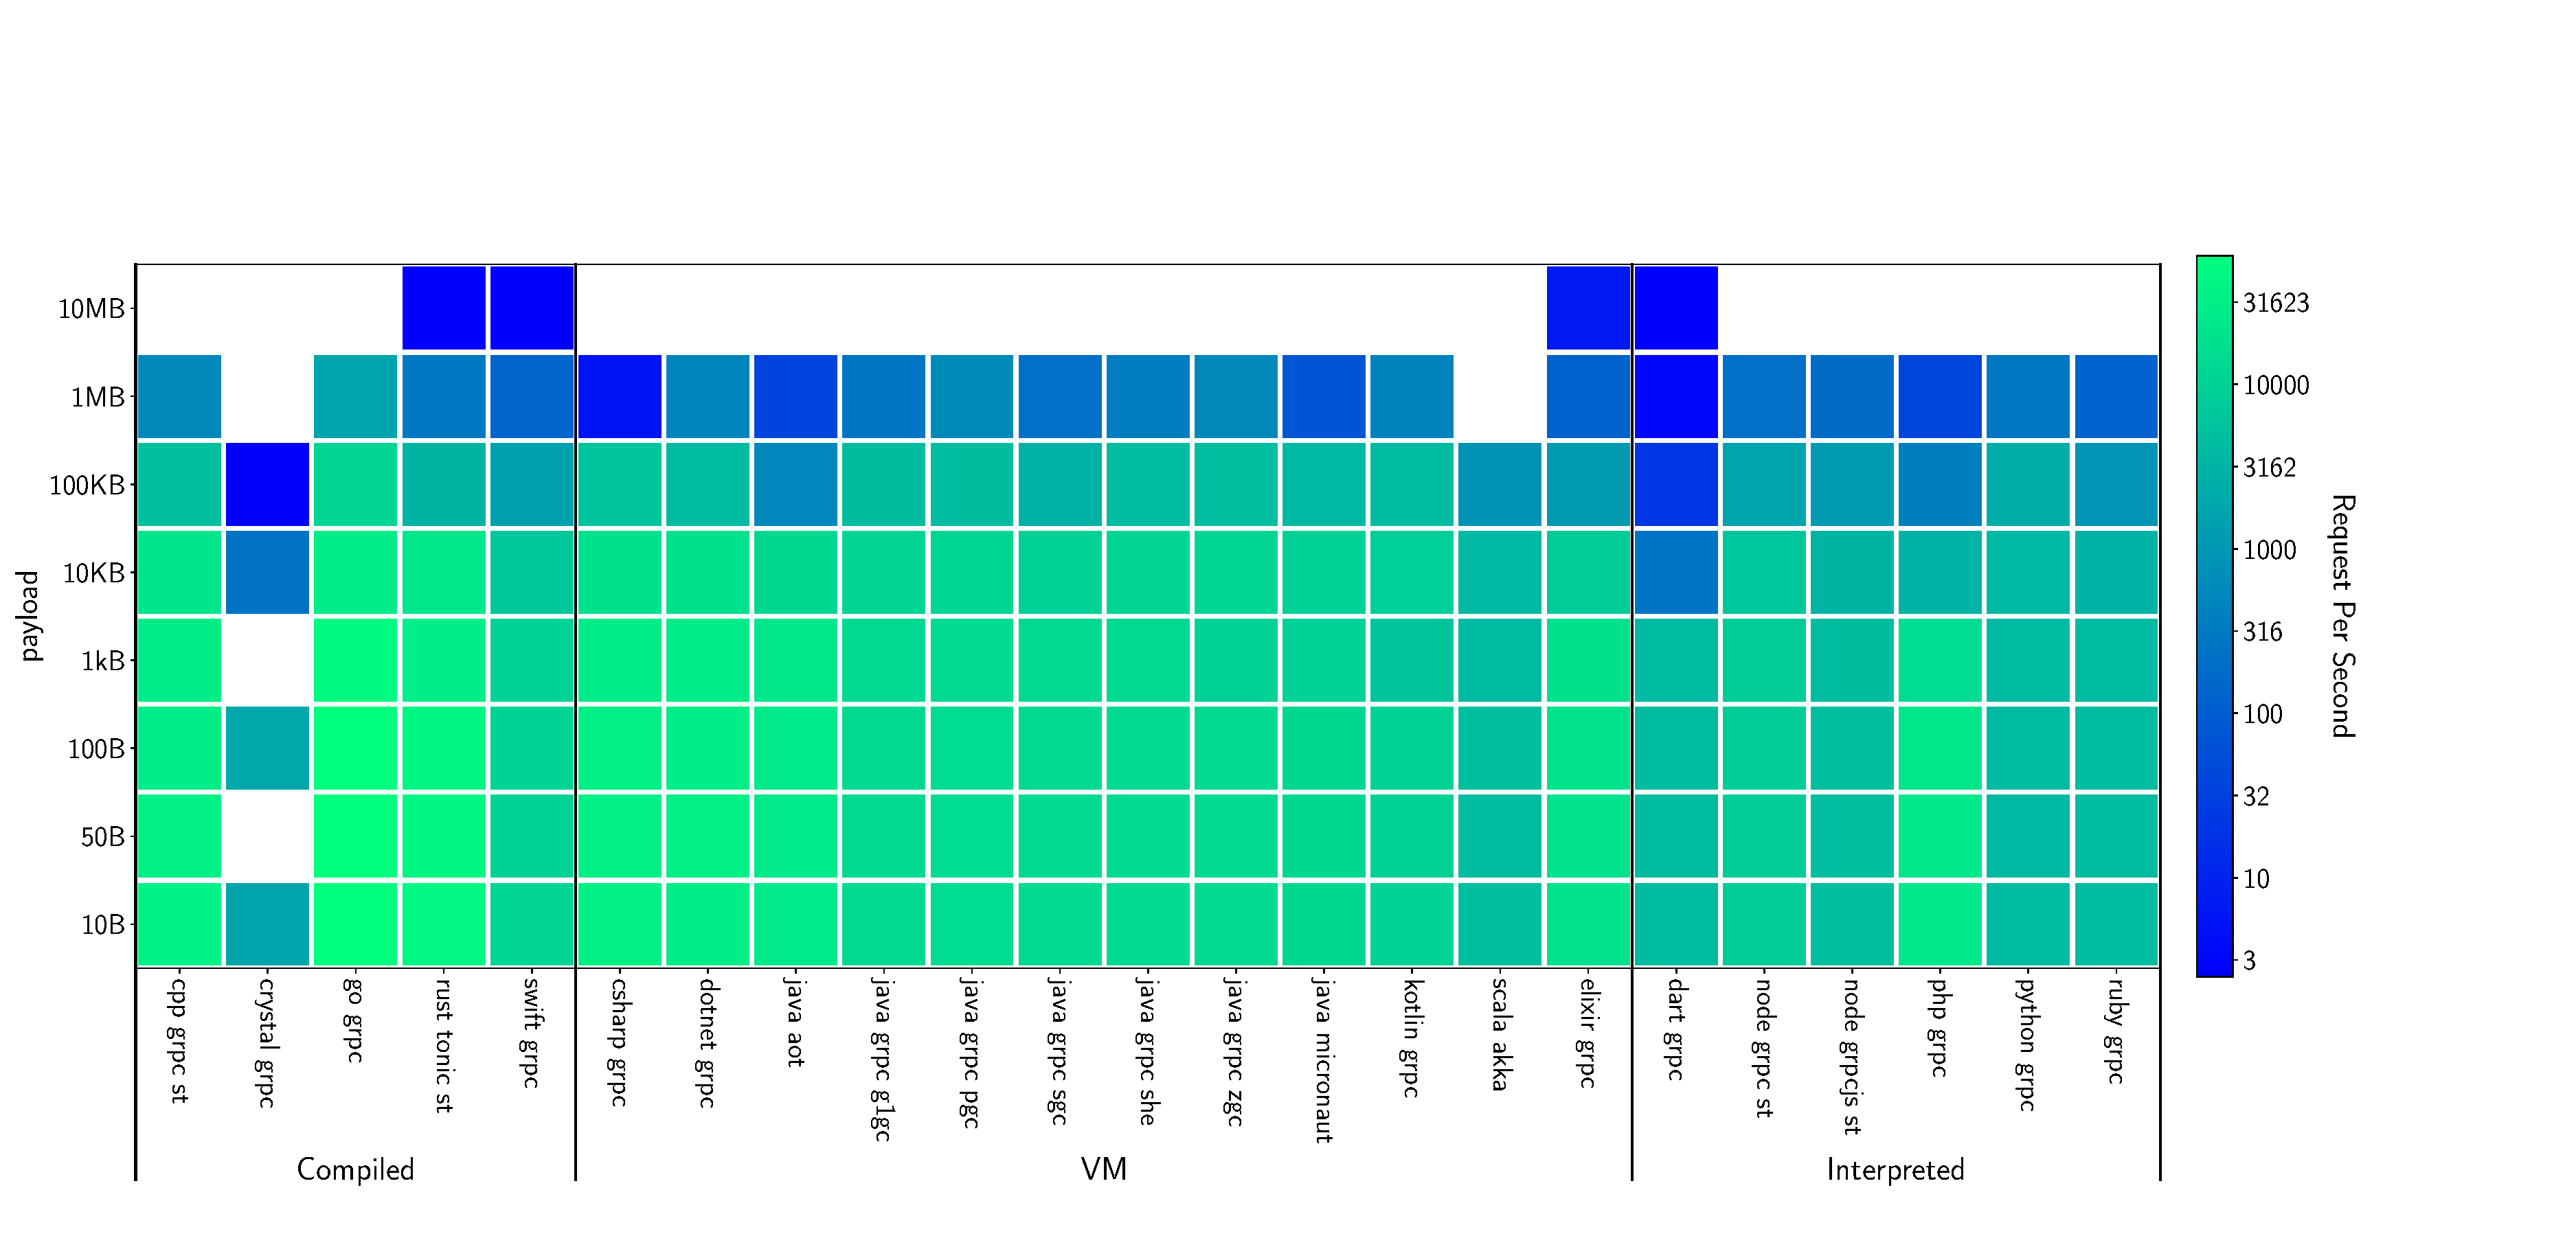
\includegraphics[width=1.2\linewidth]{imgs/rps_payload}
    \end{center}
    \caption{Number of requests per second based on the request size}\label{fig:rps_payload}
\end{figure}

\begin{figure}[!hbt]
    \begin{center}
        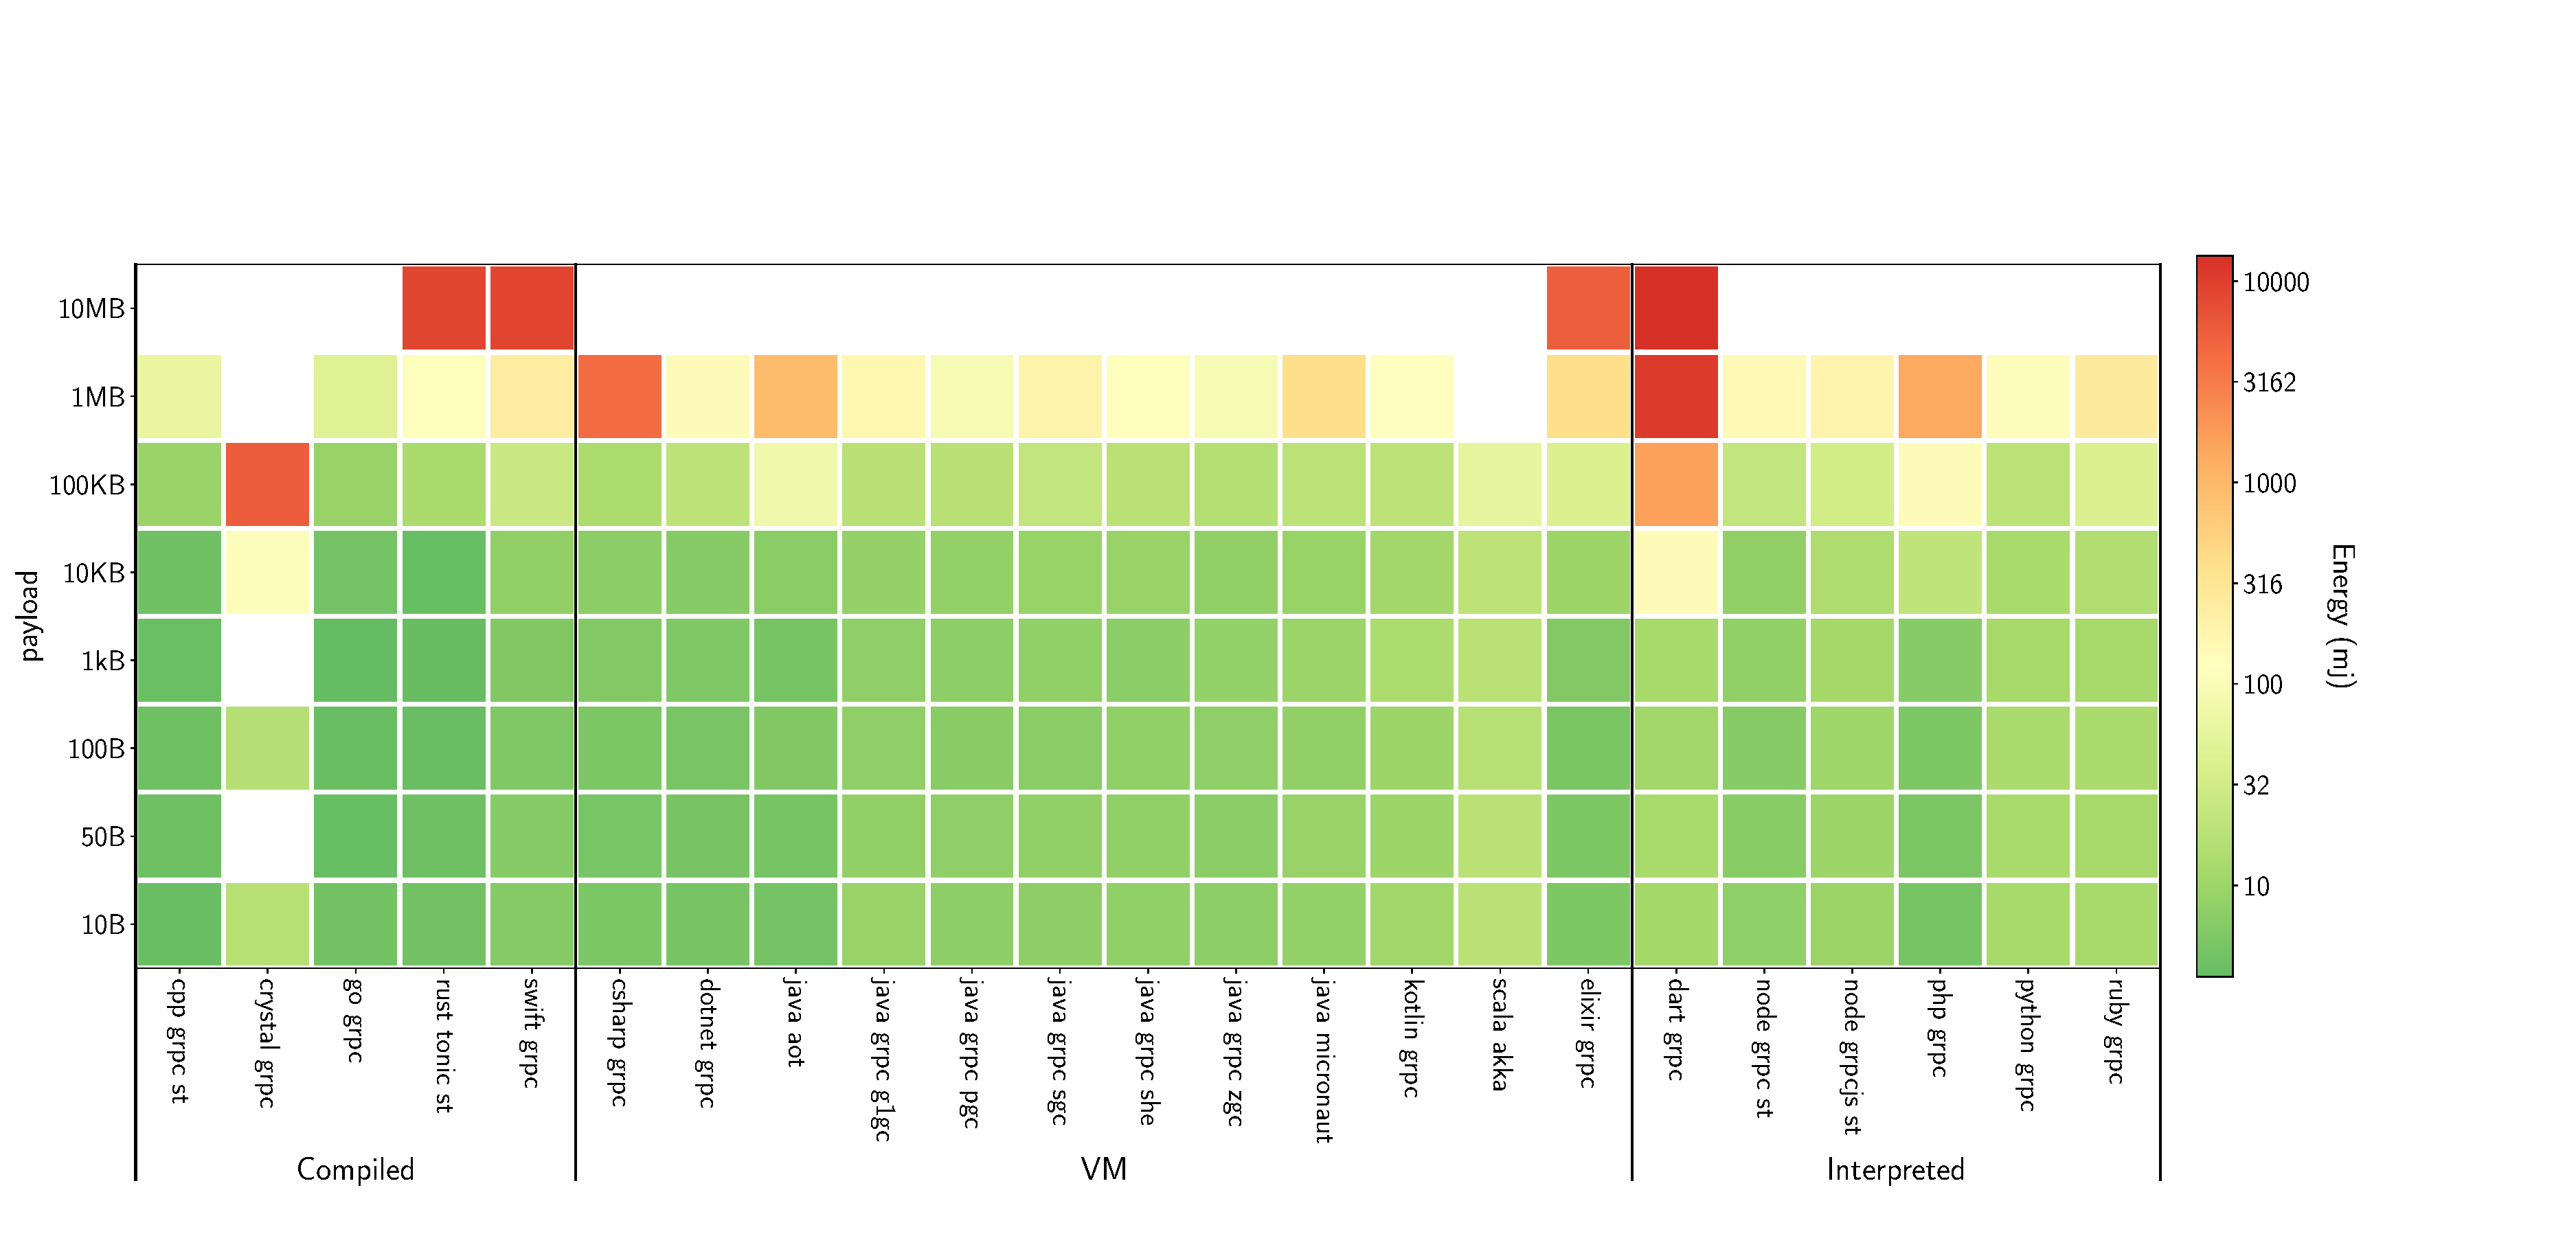
\includegraphics[width=1.2\linewidth]{imgs/energy_cost_payload}
    \end{center}
    \caption{Energy consumption based on the request size}\label{fig:energy_cost_payload}
\end{figure}

For each framework, we can distinguish three modes, and they all depend on the payload size:
\begin{enumerate}
    \item \textsf{Stress-free} mode when the server has enough resources to satisfy the requests, as they require a memory less than a certain threshold (depends on the language and the platform),
    \item \textsf{Escalation} mode when the requests tend to be bigger, but the server can still manage to handle them, at the price of a change in the energy and performance behaviors,
    \item \textsf{Broken state} mode when the size of requests exceeds 1MB, most of the servers cannot handle them, and they tend to crash. After 10MB, except for Elixir, no server could handle those requests.
\end{enumerate}


\subsubsection{Stress-Free Mode}
The compiled languages consume fewer resources (average power) in this mode.
JVM-based languages tend to consume more energy, especially Scala.
However, we do not observe the same behavior regarding efficiency.
Unlike the other interpreted programming languages, PHP's performance can be compared to the compiled ones, such as CPP or GO, and even better to others, such as Swift.
JVM-based languages tend to have better performance than interpreted ones.
Furthermore, OpenJDK has shown more efficiency than GraalVM.
Overall, we can have three groups when it comes to the cost of each request:
\begin{itemize}
    \item Energy-efficient class: C++, GO, RUST, ELIXIR, and PHP,
    \item Middle class: Most of the interpreted languages and VM-based ones,
    \item Energy-greedy class: Crystal and Scala.
\end{itemize}

\subsubsection{Escalation Mode}
In this mode, the behavior of the server depends on the payload. We observe three cases:
\begin{enumerate}
    \item drop in performances without an increased power source, such as Net core, Java Micronaut, Crystal, and Dart.
          In this case, the server uses the same resources, sometimes less, because it takes more time to handle fewer requests.
          This class of languages tends to be the most energy-consuming when it comes to the cost per request;
    \item increase in power without affecting the performance, such as Go or.Net.
          The energy consumption of a single request is affected slightly but still increases.
    \item Increase in power while dropping in performance.
          Despite the increase in power consumption, the server becomes slightly slower, which increases the energy cost per request.
          This cost is still better than the first case, which concludes that the servers in the first category are on the verge of breaking.
\end{enumerate}

We can mention the case of \textsf{Elixir} that keeps scaling despite the lack of performance compared to other compiled languages (Go, CPP).

\subsubsection{Broken state mode }
Only four of the 25 configurations could parse the 10 MB files, and only one of those could achieve a 76\% acceptance rate, which is Elixir. The other 3 had less than a 3\% success rate (Rust, Swift, and Dart).
The rest could be divided into two categories:
\begin{itemize}
    \item \textsf{Timeout} where requests took too much time that the client canceled them in this category, we find most of the dynamic codes, such as OpenJDK and Kotlin,
    \item \textsf{Size of request} exceeded the maximum size when the implementation could not handle requests with a large size, as observed with .Net, Go, .Net core, CPP, PHP, Scala, Nodejs, Ruby, and Python.
\end{itemize}


% \subsection{Threads to Validity \note{missing}}

\subsection{Summary}

This section reports on a study on the impact of programming languages on the energy for request handling.
To do that, we used an implementation of $25$ frameworks based on $17$ programming languages.
These servers use the official RPC protocol, reducing programmers' bias toward specific languages.

The results show that the number of clients had a binary effect on the servers.
With a small number of clients, there was no typical behavior between different categories.
On the other hand, when dealing with a more significant number of clients, interpreted languages and compiled ones dropped in terms of performance while keeping the same average power, unlike the VM-based ones that increased their average power while keeping the same performance.
Overall, the second strategy had a better impact on the single request cost than the first one.

As for the evolution of the query size, we have seen three modes of behavior for each framework, depending on the size of the requests: the stress-free mode, the escalation mode, and the broken state mode.
We start with the stress-free mode.
The leader class was the compiled languages, while the VM-based ones tended to consume more energy.
Finally, with the escalation mode, one could observe three strategies to deal with the increase in request size.
The first strategy tends to drop performances while consuming the same power; the second was to increase the average power consumption without impacting the performances; the third was a combination of both previous strategies with an increase in power and a drop in performance.
Interestingly, the third strategy had a lower cost per request than the first one.
Finally, most implementations could not handle requests heavier than 10 MB for the broken mode.
Elixir was an exception to this limit despite its low performance compared to other languages.

This study shows the absence of a universal language when dealing with RPC requests.
Moreover, each implementation had a different way of dealing with scalability.
While some chose to increase the average power consumption, others dropped in performance.
Both of these strategies led to a higher cost of a single request.

\clearpage